\section{A practical fault detection scheme}
The oracle-based detection scheme described in Section~\ref{sec:faultDetection} gives good results, however, it cannot be implemented for several reasons. First, the error $\|{w}_{f+1} - \widetilde{w}_{f+1}\|$ cannot be measured directly, since $w_{f+1}$ is not available, only $\widetilde{w}_{f+1}$ is. An approximation for the error is proposed and evaluated in~\ref{sec:checksum}. Second, the threshold $\tau_c = c \cdot \varepsilon / |\widetilde{y}_{\ell, f}|$ requires the $\widetilde{y}_{\ell, f}$ vector which is computed at the last iteration $\ell$ of the execution, and is then not yet available at the fault iteration, so an approximation is also proposed and evaluated in~\ref{sec:threshold}. Moreover, the iteration when the fault occurred is not known either, but this issue can easily be taken care of by applying the scheme at each iteration, and replacing $f$ by the current iteration index $i$ as described in~\ref{sec:practical_scheme}. Finally, the new implementable scheme is evaluated in~\ref{sec:implementable_evaluated}.

\subsection{Estimation of the error using a check-sum approach}\label{sec:checksum}
Traditional approaches for detecting transient faults in SpMV product include check-sums \cite{checksum}. The main idea of such techniques is to encode some data, here the Matrix A data, with the vector $\allOne^T = (1, 1,..., 1)$, to perform the same operations on the encoded data, which are usually much cheaper than the operations on the real data, and to check the result consistency (result on encoded data = encoded result on real data). Assuming exact arithmetic and no error happened during the operations on encoded data, a wrong result often implies a faulty execution. 
In exact arithmetic, the following equations hold :


\begin{equation}
%
    \begin{pmatrix}
        A  \\
        \allOne^T \cdot A 
     \end{pmatrix} \cdot
	v
    =  \begin{pmatrix}
        A \cdot v \\
        (\allOne^T \cdot A) \cdot v
     \end{pmatrix} 
    =  \begin{pmatrix}
        A \cdot v \\
        \allOne^T \cdot (A \cdot v)
     \end{pmatrix} 
%
\end{equation}

In case of a fault in A ($reg_1$), the previous equation becomes:

\begin{equation}
%
    \begin{pmatrix}
        \widetilde{A}  \\
        \allOne^T \cdot A 
     \end{pmatrix} \cdot
	v
    =  \begin{pmatrix}
        \widetilde{A} \cdot v \\
        (\allOne^T \cdot A) \cdot v
     \end{pmatrix} 
    \neq  \begin{pmatrix}
        \widetilde{A} \cdot v \\
        \allOne^T \cdot (\widetilde{A} \cdot v)
     \end{pmatrix} 
%
\end{equation}
The difference between the result on encoded data and the encoded result $|(\allOne^T \cdot A)^T v - \allOne^T (\widetilde{A} \cdot v)|$ is called the check-sum,
where $\allOne^T \cdot A$ is a row vector computed once with  its $j^{th}$ entry is the sum of all entries of the $j^{th}$ row of $A$.
Then, in exact arithmetic we have: 
\begin{equation} \label{eqn:checksum}
 \text{check-sum = } |(\allOne^T \cdot A)^T  v - \allOne^T (\widetilde{A} \cdot v)| = |\allOne^T (w-\widetilde{w})| = \|w - \widetilde{w}\|
\end{equation}
 If no fault occurred, $w = \widetilde{w}$ and the check-sum is equal to 0, whereas if a fault occurred, the check-sum is equal to the error introduced by the fault. The same method holds if the fault occurred in another register, and for preconditioned-GMRES (by replacing in the previous equations $v$ by $z = M^{-1} \cdot v$). 

However, because all calculations are performed using floating point arithmetic; the previous equations do not hold anymore due to rounding errors (and the loss of associativity).
Only an approximation of $\|w - \widetilde{w} \|$ can be obtained from Equation~\eqref{eqn:checksum}.
Figure~\ref{fig:conv_hist_checksum} plots the check-sum computed at each iteration i for different bit-flips and compares it to the true error $\|w_i - \widetilde{w}_i \|$. In Figure~\ref{fig:gre_216a_conv_hist_checksum_0}, the effect of the fault on the check-sum is not distinguishable from the rounding errors, as the register's $60^{th}$ bit is flipped, causing an extremely small error. In Figure~\ref{fig:gre_216a_conv_hist_checksum_1} and Figure~\ref{fig:gre_216a_conv_hist_checksum_2}, in which bit 50 and bit 40 are flipped respectively, a peak can be seen at the fault iteration and visually differentiated from the check-sum fluctuations. We observe that for a relatively small matrix like gre_216a, the check-sum accuracy is approximately $10^{-15}$ whereas in the case of a larger matrix such as pores_2, more rounding errors accumulates, up to $10^{-10}$. Hence faults causing small errors (such as in figures~\ref{fig:pores_2_conv_hist_checksum_0} and ~\ref{fig:pores_2_conv_hist_checksum_1} where the bit 50 and the bit 40 are flipped respectively) can hardly be distinguished from the check-sum fluctuations, and the true error is not approximated very accurately.

To conclude, the check-sum described in Equation \eqref{eqn:checksum} seems to be a good approximation of the error, but may loose in accuracy as the matrix size increases, making small faults harder to detect.
%TODO
%is a critical fault or   One way to automatically distinguish between the occurrence of a fault and rounding errors is to use the threshold established in the previous section. By Previous observations show that some iterations are more sensible than others (for example the first iterations), so the threshold should ideally be computed at each iteration and reflects the iteration sensibility.



\begin{figure}[h]
	\centering
    
\begin{minipage}[b]{0.45\linewidth}
\centering
\textbf{GMRES} executions on \textbf{gre_216a} 
\end{minipage}
\quad
\begin{minipage}{0.45\linewidth}
\centering
\textbf{preconditioned-GMRES} on \textbf{pores_2}
\end{minipage}\\


    \begin{minipage}[b]{0.48\linewidth}
	\begin{subfigure}[t]{\linewidth}
		\centering
		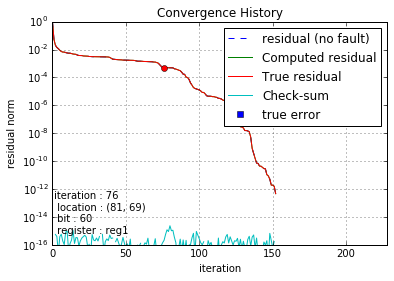
\includegraphics[width=\linewidth]{figures/gre_216a/convergence_history_checksum_0.png}
		\caption{}\label{fig:gre_216a_conv_hist_checksum_0}		
	\end{subfigure}
	\quad
	\begin{subfigure}[t]{\linewidth}
		\centering
		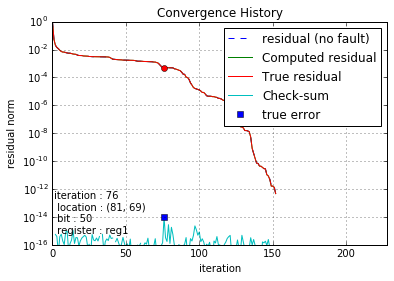
\includegraphics[width=\linewidth]{figures/gre_216a/convergence_history_checksum_1.png}
		\caption{}\label{fig:gre_216a_conv_hist_checksum_1}
	\end{subfigure}
    \quad
    \begin{subfigure}[t]{\linewidth}
		\centering
		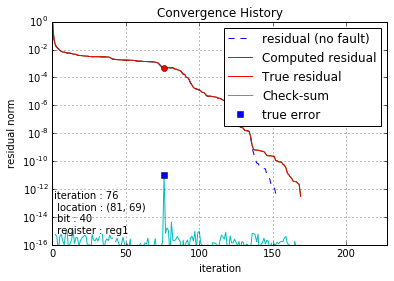
\includegraphics[width=\linewidth]{figures/gre_216a/convergence_history_checksum_2.png}
		\caption{}\label{fig:gre_216a_conv_hist_checksum_2}
	\end{subfigure}
    \end{minipage}
    \quad
    \begin{minipage}[b]{0.48\linewidth}
    	\begin{subfigure}[t]{\linewidth}
		\centering
		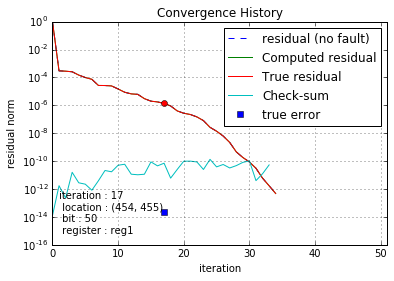
\includegraphics[width=\linewidth]{figures/pores_2/convergence_history_checksum_0.png}
		\caption{}\label{fig:pores_2_conv_hist_checksum_0}		
	\end{subfigure}
	\quad
	\begin{subfigure}[t]{\linewidth}
		\centering
		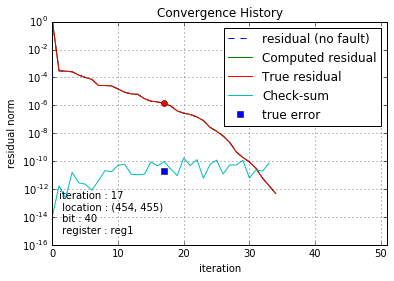
\includegraphics[width=\linewidth]{figures/pores_2/convergence_history_checksum_1.png}
		\caption{}\label{fig:pores_2_conv_hist_checksum_1}
	\end{subfigure}
    \quad
    \begin{subfigure}[t]{\linewidth}
		\centering
		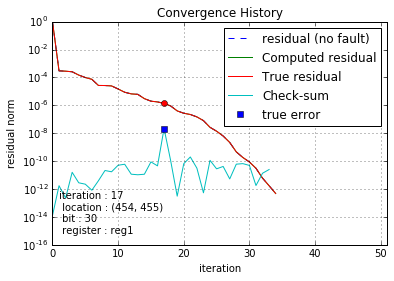
\includegraphics[width=\linewidth]{figures/pores_2/convergence_history_checksum_2.png}
		\caption{}\label{fig:pores_2_conv_hist_checksum_2}
	\end{subfigure}

    
	\end{minipage}
\caption{Convergence histories of 3 GMRES executions on HB/gre_216a and 3 preconditioned-GMRES executions on HB/pored_2, disrupted by a transient fault. The check-sum at each iteration is plotted, as well as the true error denoted by a blue square.} %TODO 
\label{fig:conv_hist_checksum}
\end{figure}






\subsection{Approximation of the threshold and evaluation}\label{sec:threshold}
Based on the observation that $\widetilde{y}_{j, i}$ usually remains nearly constant as $j$ increases. We will used $\widetilde{y}_{i, i}$ at each iteration $i$ to compute an approximated threshold. This observation does not seem to benefit from much theoretical attention but is supported by the intuition that the solution's directions are mainly determined by the first iteration, whereas the latter iterations are responsible for their refinement. Figure~\ref{fig:conv_hist_threshold_evaluation} compares the true check-sum to the approximated one. In each cases, the two curves do not overlap perfectly, nevertheless the general trend of the true threshold seems to be followed by its implementable approximation.



\begin{figure}[h]
	\centering
    
\begin{minipage}[b]{0.45\linewidth}
\centering
\textbf{GMRES} executions on \textbf{gre_216a} 
\end{minipage}
\quad
\begin{minipage}{0.45\linewidth}
\centering
\textbf{preconditioned-GMRES} on \textbf{pores_2}
\end{minipage}\\


    \begin{minipage}[b]{0.48\linewidth}
	
	\begin{subfigure}[t]{\linewidth}
		\centering
		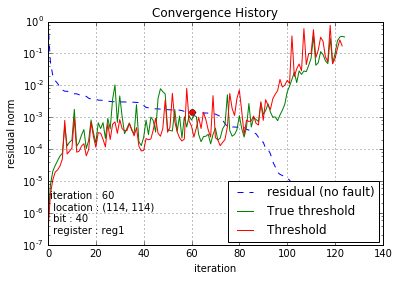
\includegraphics[width=1.1\linewidth]{figures/gre_216a/convergence_history_threshold_evaluation_0.png}
		\caption{$\varepsilon = 10^{-6}$}\label{fig:gre_216a_conv_hist_threshold_evaluation_0}	
	\end{subfigure}
    \quad
    \begin{subfigure}[t]{\linewidth}
		\centering
		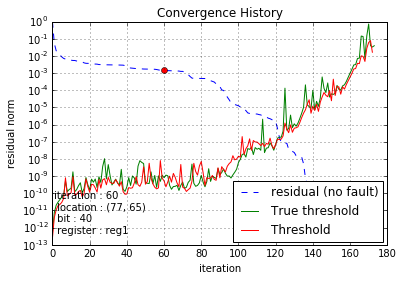
\includegraphics[width=1.1\linewidth]{figures/gre_216a/convergence_history_threshold_evaluation_1.png}
		\caption{$\varepsilon = 10^{-12}$}\label{fig:gre_216a_conv_hist_threshold_evaluation_1}	
	\end{subfigure}
    \end{minipage}
    \quad
    \begin{minipage}[b]{0.48\linewidth}
    	
	\begin{subfigure}[t]{\linewidth}
		\centering
		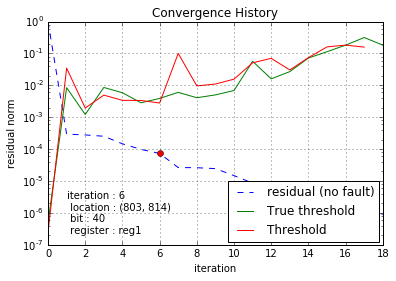
\includegraphics[width=1.1\linewidth]{figures/pores_2/convergence_history_threshold_evaluation_0.png}
		\caption{$\varepsilon = 10^{-6}$}\label{fig:pores_2_conv_hist_threshold_evaluation_0}	
	\end{subfigure}
    \quad
    \begin{subfigure}[t]{\linewidth}
		\centering
		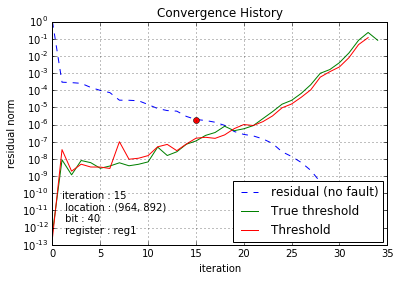
\includegraphics[width=1.1\linewidth]{figures/pores_2/convergence_history_threshold_evaluation_1.png}
		\caption{$\varepsilon = 10^{-12}$}\label{fig:pores_2_conv_hist_threshold_evaluation_1}	
	\end{subfigure}

	\end{minipage}
\caption{Convergence histories of a GMRES execution on HB/gre_216a and a preconditioned-GMRES executions on HB/pored_2 for two target accuracies ($\varepsilon = 10^{-6}$ and $\varepsilon = 10^{-12}$). The true threshold ($c \cdot \varepsilon / |\widetilde{y}_{\ell, i}|$) and the approximation ($c \cdot \varepsilon / |\widetilde{y}_{i, i}|$) are compared. Even though the curves do not perfectly overlap, the general evolution of the true threshold seems to be preserved in the approximated one.}\label{fig:conv_hist_threshold_evaluation}
\end{figure}




\subsection{Implementation of the practical scheme}\label{sec:practical_scheme}
Let $0 < c < 1$. To sum up, here is the practical implementable scheme. 
\begin{enumerate}
\item The target accuracy is set to $(1-c)\cdot \varepsilon$. 
\item At the beginning of the execution, the matrix A data is encoded with $\allOne^T$
\item At each iteration i, check-sum(i) and $\tau_c(i)\textprime = c \cdot \varepsilon / \widetilde{y}_{i, i}$ are computed
\item The following test is performed $$ \text{check-sum(i)} < \tau_c(i)\textprime = c \cdot \varepsilon / \widetilde{y}_{i, i}$$
\item If the test is true, then no fault is detected, otherwise the detection is triggered.
\end{enumerate}


Since the detection is performed at each iteration, the outcome naming needs to be updated (Table \ref{colors}). a detection is said to be correct when it happened at the exact iteration when the fault occurred, whereas a detection triggered at any iteration different from the faulty one is said to be incorrect.

\begin{table}[h]
\centering
\caption{New set of outcomes and their colors.}
\label{colors}
\begin{tabular}{l|ll|}
	& Convergence & No convergence\\
    \hline
   Correct detection & \color[RGB]{30, 30, 30}{\textbf{No impact fault detected}} & \color[RGB]{85, 147, 47}{\textbf{Critical fault detected}} \\
  
   Incorrect detection & \color{orange}{\textbf{Incorrect detection}} & \color{orange}{\textbf{Incorrect detection}} \\
   No detection & \color[RGB]{90, 90, 90}{\textbf{No impact fault ignored}} & \color{red}{\textbf{Critical fault ignored}} \\
    \hline
\end{tabular}
\end{table}

 In Figure \ref{fig:conv_hist_threshold}, the approximated threshold $\tau_{0.5}$ and the check-sum are plotted at each iteration for 2 GMRES executions disrupted by a fault. In Figure \ref{fig:gre_216a_conv_hist_threshold_0}, the check-sum at the fault iteration is smaller than the threshold, so the fault is not detected, and the execution does converge, which produce a \emph{No impact fault ignored} from Table~\ref{colors}. In Figure~\ref{fig:gre_216a_conv_hist_threshold_2}, the check-sum is greater than the threshold at the fault iteration and the execution does not converge, which produce a \emph{Critical fault detected} from Table~\ref{colors}. 

However in Figure \ref{fig:conv_hist_threshold_false}, two convergence histories of executions disrupted by an incorrectly detected fault are plotted for GMRES and preconditioned-GMRES. In Figure \ref{fig:gre_216a_conv_hist_threshold_3}, check-sum(i) remains below $\tau_{0.5}(i)$ so the fault is undetected, even though the execution does not converge, which correspond to a \emph{Critical fault not detected} from Table \ref{colors}. In Figure \ref{fig:gre_216a_conv_hist_threshold_4}, check-sum(i) exceeds $\tau_{0.5}(i)$ at the fault iteration so a fault is detected, but the execution still converges which correspond to a \emph{No impact fault detected} from Table \ref{colors}. 



\begin{figure}[h]
	\centering
    
\begin{minipage}[b]{0.45\linewidth}
\centering
\textbf{-GMRES} executions on \textbf{gre_216a} 
\end{minipage}
\quad
\begin{minipage}{0.45\linewidth}
\centering
\textbf{preconditioned-GMRES} on \textbf{pores_2}
\end{minipage}\\


    \begin{minipage}[b]{0.48\linewidth}
	
	\begin{subfigure}[t]{\linewidth}
		\centering
		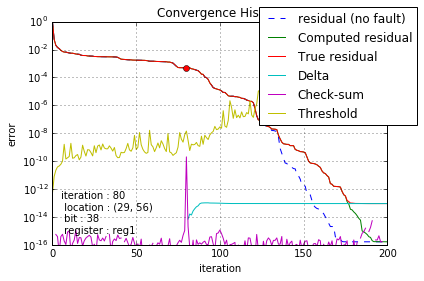
\includegraphics[width=\linewidth]{figures/gre_216a/convergence_history_threshold_0.png}
		\caption{No impact fault ignored}\label{fig:gre_216a_conv_hist_threshold_0}
	\end{subfigure}
    \quad
    \begin{subfigure}[t]{\linewidth}
		\centering
		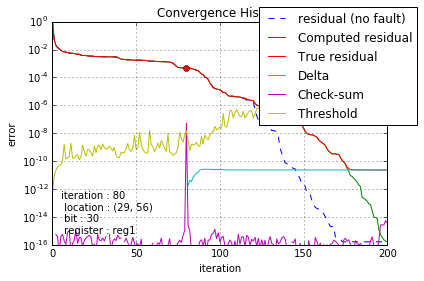
\includegraphics[width=\linewidth]{figures/gre_216a/convergence_history_threshold_2.png}
		\caption{Critical fault detected}\label{fig:gre_216a_conv_hist_threshold_2}
	\end{subfigure}
    \end{minipage}
    \quad
    \begin{minipage}[b]{0.48\linewidth}
    	
	\begin{subfigure}[t]{\linewidth}
		\centering
		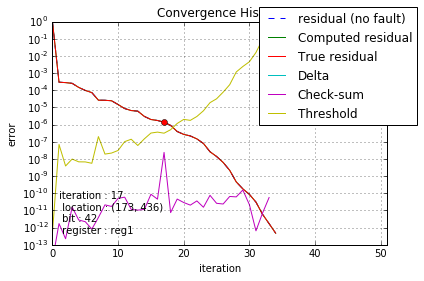
\includegraphics[width=\linewidth]{figures/pores_2/convergence_history_threshold_0.png}
		\caption{No impact fault ignored}\label{fig:pores_2_conv_hist_threshold_0}
	\end{subfigure}
    \quad
    \begin{subfigure}[t]{\linewidth}
		\centering
		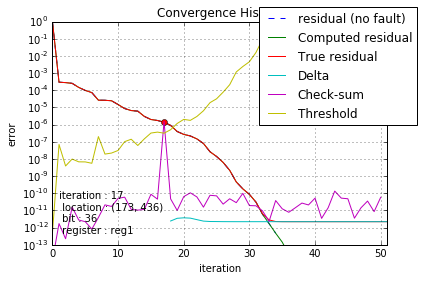
\includegraphics[width=\linewidth]{figures/pores_2/convergence_history_threshold_2.png}
		\caption{Critical fault detected}\label{fig:pores_2_conv_hist_threshold_2}
	\end{subfigure}

    
	\end{minipage}
\caption{Convergence histories of 2 GMRES executions on HB/gre_216a and 2 preconditioned-GMRES executions on HB/pored_2, disrupted by transient faults that are properly detected. The check-sum and the threshold at each iteration are plotted. In figures~\ref{fig:gre_216a_conv_hist_threshold_0} and ~\ref{fig:pores_2_conv_hist_threshold_0}, the check-sum at each iteration remains below the threshold, so no fault is detected and the executions converge, producing a \emph{No impact fault ignored} from Table \ref{colors} in both cases. In figures~\ref{fig:gre_216a_conv_hist_threshold_2} and ~\ref{fig:pores_2_conv_hist_threshold_2}, the check-sum becomes higher than the threshold at the fault iteration, so the faults are detected and the executions do not converge, producing a \emph{Critical fault detected} from Table \ref{colors} in both cases. }\label{fig:conv_hist_threshold}
\end{figure}








\begin{figure}[h]
	\centering
    
\begin{minipage}[b]{0.45\linewidth}
\centering
\textbf{GMRES} executions on \textbf{gre_216a} 
\end{minipage}
\quad
\begin{minipage}{0.45\linewidth}
\centering
\textbf{preconditioned-GMRES} on \textbf{pores_2}
\end{minipage}\\


    \begin{minipage}[b]{0.48\linewidth}
	
	\begin{subfigure}[t]{\linewidth}
		\centering
		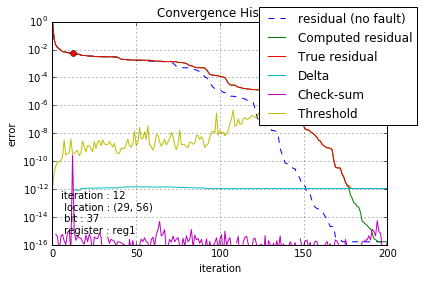
\includegraphics[width=\linewidth]{figures/gre_216a/convergence_history_threshold_3.png}
		\caption{Critical fault ignored}\label{fig:gre_216a_conv_hist_threshold_3}
	\end{subfigure}
    \quad
    \begin{subfigure}[t]{\linewidth}
		\centering
		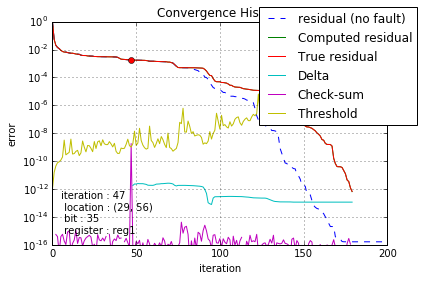
\includegraphics[width=\linewidth]{figures/gre_216a/convergence_history_threshold_4.png}
		\caption{No impact fault detected}\label{fig:gre_216a_conv_hist_threshold_4}
	\end{subfigure}
    \end{minipage}
    \quad
    \begin{minipage}[b]{0.48\linewidth}
    	
	\begin{subfigure}[t]{\linewidth}
		\centering
		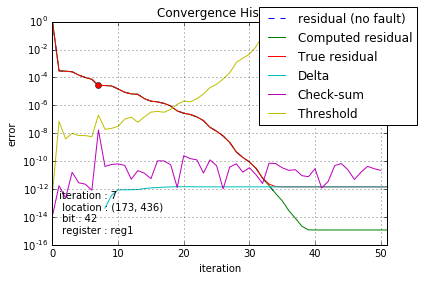
\includegraphics[width=\linewidth]{figures/pores_2/convergence_history_threshold_3.png}
		\caption{Critical fault ignored}\label{fig:pores_2_conv_hist_threshold_3}
	\end{subfigure}
    \quad
    \begin{subfigure}[t]{\linewidth}
		\centering
		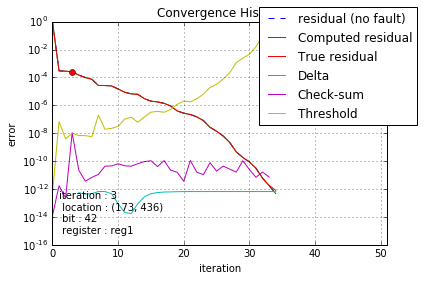
\includegraphics[width=\linewidth]{figures/pores_2/convergence_history_threshold_4.png}
		\caption{No impact fault detected}\label{fig:pores_2_conv_hist_threshold_4}
	\end{subfigure}

    
	\end{minipage}
\caption{Convergence histories of 2 GMRES executions on HB/gre_216a and 2 preconditioned-GMRES executions on HB/pored_2, disrupted by transient faults that are not properly detected. In figures~\ref{fig:gre_216a_conv_hist_threshold_3} and ~\ref{fig:pores_2_conv_hist_threshold_3}, the check-sum at each iteration remains below the threshold, so no fault is detected and the executions do not converge, producing a \emph{Critical fault ignored} from Table \ref{colors} in both cases. In figures~\ref{fig:gre_216a_conv_hist_threshold_4} and ~\ref{fig:pores_2_conv_hist_threshold_4}, the check-sum becomes slightly higher than the threshold at the fault iteration, so the faults are detected but the executions converge anyway, producing a \emph{No impact fault detected} from Table \ref{colors} in both cases. }\label{fig:conv_hist_threshold_false}
\end{figure}



This scheme requires some additional operations to be performed, mainly caused by the check-sum computation. First, since the target accuracy is set to $(1-c)\cdot \varepsilon < \varepsilon$, some additional iterations $\widetilde{\ell}-\ell$ may be required for the execution to converge. Second, the quantity $ \allOne^T \cdot A$ is computed once at the beginning, and requires $\Theta(nnz)$ (number of nonzero elements in A) operations. Then, at each iteration, the vectors  $(\allOne^T \cdot A) \cdot v$ and $\allOne^T \cdot (A \cdot v)$ as well as their Euclidean distance are computed, necessitating at each iteration $\Theta(n)$ operations. Finally, $\Theta(1)$ operations are needed for the $\text{check-sum} < \text{threshold}$ comparison. Therefore, the test requires $\Theta(nnz) + \Theta(n \cdot \widetilde{\ell})$ additional operations, negligible when compared to the $\Theta(\ell \cdot nnz)$ operations of the classical algorithm, as long as $n \ll nnz$ and $\widetilde{\ell} \approx \ell$. Moreover, those computations can be performed in parallel in a separate computation unit since their outputs are not used in the classical execution.


\subsection{Evaluation of the practical detection scheme}\label{sec:implementable_evaluated}
%TODO
Figure~\ref{fig:test_result} plots the proportion (\% of executions) of detection scheme outcomes for several values of $c$. Because of the previously described approximations, Theorem~\ref{theorem} does not hold anymore and some \emph{Critical fault ignored} are produced. Except for the preconditioned-GMRES case in low accuracy ($\varepsilon = 10^{-6}$), the detection scheme does perform well as the proportion of critical fault missed is relatively low. For more details, the $c=0.5$ cases are plotted in Figure~\ref{fig:test_result_c05} and in Figure~\ref{fig:test_result_c05_matrices} for the results on the matrix set. However, the case preconditioned-GMRES in low accuracy is worrying. To understand why the test performed poorly in this situation, Figure~\ref{fig:why} plots the approximated threshold and check-sum in the case of an important fault inducing a large error. We can see that in both plots, the fault increases significantly the threshold, disrupting the convergence (which never seems to happen in GMRES executions without preconditioner). This problem comes from the approximation on $\widetilde{y}_{l, f} \rightarrow \widetilde{y}_{f, f}$, so another approximation should probably be established to ensure better results in various inputs.
%TODO: expliquer les figures



\begin{figure}[h]
	\centering
    
\begin{minipage}[b]{0.45\linewidth}
\centering
\textbf{GMRES} executions on \textbf{gre_216a} 
\end{minipage}
\quad
\begin{minipage}{0.45\linewidth}
\centering
\textbf{preconditioned-GMRES} on \textbf{pores_2}
\end{minipage}\\


    \begin{minipage}[b]{0.48\linewidth}
	
	\begin{subfigure}[t]{\linewidth}
		\centering
		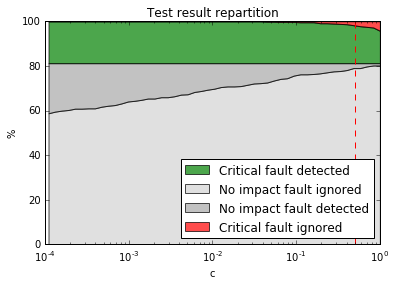
\includegraphics[width=1.1\linewidth]{figures/gre_216a/test_result_0.png}
		\caption{$\varepsilon = 10^{-6}$}\label{fig:gre_216a_test_result_0}	
	\end{subfigure}
    \quad
    \begin{subfigure}[t]{\linewidth}
		\centering
		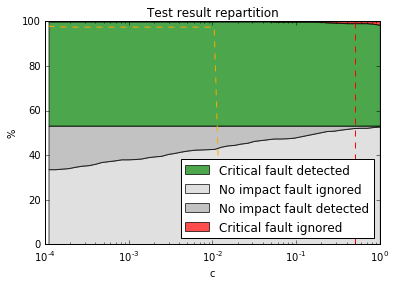
\includegraphics[width=1.1\linewidth]{figures/gre_216a/test_result_1.png}
		\caption{$\varepsilon = 10^{-12}$}\label{fig:gre_216a_test_result_1}	
	\end{subfigure}
    \end{minipage}
    \quad
    \begin{minipage}[b]{0.48\linewidth}
    	
	\begin{subfigure}[t]{\linewidth}
		\centering
		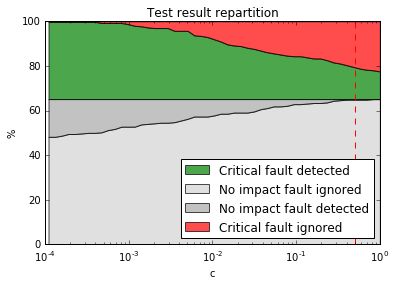
\includegraphics[width=1.1\linewidth]{figures/pores_2/test_result_0.png}
		\caption{$\varepsilon = 10^{-6}$}\label{fig:pores_2_test_result_0}	
	\end{subfigure}
    \quad
    \begin{subfigure}[t]{\linewidth}
		\centering
		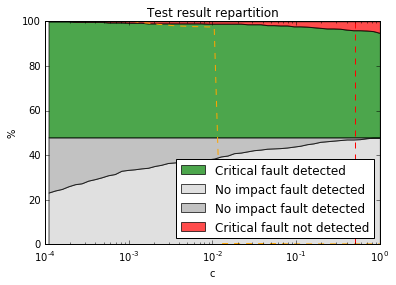
\includegraphics[width=1.1\linewidth]{figures/pores_2/test_result_1.png}
		\caption{$\varepsilon = 10^{-12}$}\label{fig:pores_2_test_result_1}	
	\end{subfigure}

	\end{minipage}
\caption{Diagrams representing the test outcome proportion for several values of c. To compute them, faulty executions covering a large part of the fault parameter space were performed. The case $c = 0.5$ represented by the dashed red line is detailed in Figure~\ref{fig:test_result_c05}. The dashed orange line corresponds to the proportion of execution where an incorrect detection happens.}\label{fig:test_result}
\end{figure}




\begin{figure}[h]
	\centering
    
\begin{minipage}[b]{0.45\linewidth}
\centering
\textbf{GMRES} executions on \textbf{gre_216a} 
\end{minipage}
\quad
\begin{minipage}{0.45\linewidth}
\centering
\textbf{preconditioned-GMRES} on \textbf{pores_2}
\end{minipage}\\


    \begin{minipage}[b]{0.48\linewidth}
	
	\begin{subfigure}[t]{\linewidth}
		\centering
		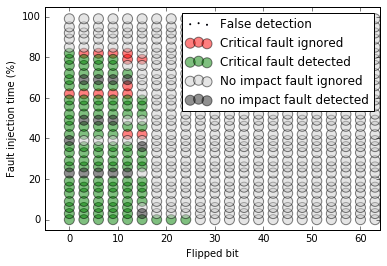
\includegraphics[width=1.1\linewidth]{figures/gre_216a/test_result_c05_0.png}
		\caption{$\varepsilon = 10^{-6}$}\label{fig:gre_216a_test_result_c05_0}	
	\end{subfigure}
    \quad
    \begin{subfigure}[t]{\linewidth}
		\centering
		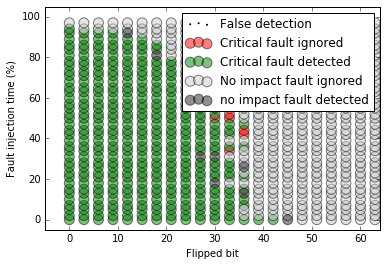
\includegraphics[width=1.1\linewidth]{figures/gre_216a/test_result_c05_1.png}
		\caption{$\varepsilon = 10^{-12}$}\label{fig:gre_216a_test_result_c05_1}	
	\end{subfigure}
    \end{minipage}
    \quad
    \begin{minipage}[b]{0.48\linewidth}
    	
	\begin{subfigure}[t]{\linewidth}
		\centering
		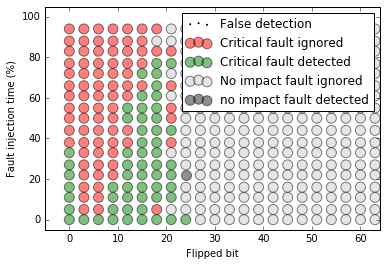
\includegraphics[width=1.1\linewidth]{figures/pores_2/test_result_c05_0.png}
		\caption{$\varepsilon = 10^{-6}$}\label{fig:pores_2_test_result_c05_0}	
	\end{subfigure}
    \quad
    \begin{subfigure}[t]{\linewidth}
		\centering
		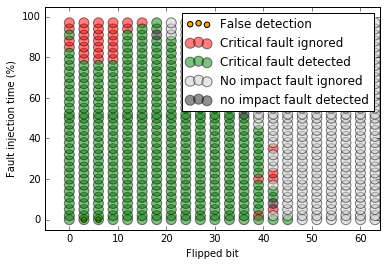
\includegraphics[width=1.1\linewidth]{figures/pores_2/test_result_c05_1.png}
		\caption{$\varepsilon = 10^{-12}$}\label{fig:pores_2_test_result_c05_1}	
	\end{subfigure}

	\end{minipage}
\caption{Diagram detailing the test results for $c = 0.5$. Each dot corresponds to a faulty execution, and its color represents the test outcome.}
\label{fig:test_result_c05}
\end{figure}



\begin{figure}[h]
	\centering

    \begin{minipage}[b]{0.48\linewidth}
	
    \begin{subfigure}[t]{\linewidth}
		\centering
		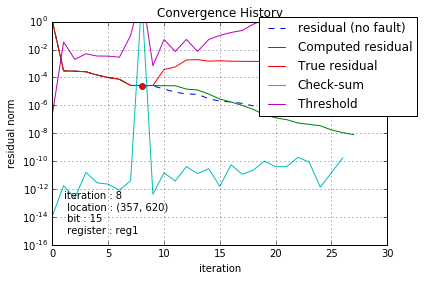
\includegraphics[width=1.1\linewidth]{figures/pores_2/convergence_history_problem_1.png}
		\caption{$\varepsilon = 10^{-12}$}\label{fig:gre_216a_test_result_1}	
	\end{subfigure}
    \end{minipage}
    \quad
    \begin{minipage}[b]{0.48\linewidth}
    	
	
    \begin{subfigure}[t]{\linewidth}
		\centering
		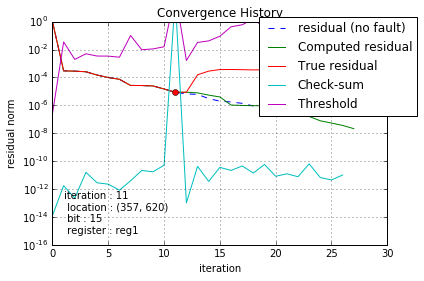
\includegraphics[width=1.1\linewidth]{figures/pores_2/convergence_history_problem_0.png}
		\caption{$\varepsilon = 10^{-12}$}\label{fig:pores_2_test_result_1}	
	\end{subfigure}

	\end{minipage}
\caption{Two convergence histories of preconditioned-GMRES on pores_2, disrupted by a large fault (bit 15). The error is so important that it modifies significantly the threshold, disrupting the detection scheme.}\label{fig:test_result}
\end{figure}\label{fig:why}






\begin{figure}[h]
	\centering
    
\begin{minipage}[b]{0.45\linewidth}
\centering
\textbf{GMRES} executions
\end{minipage}
\quad
\begin{minipage}{0.45\linewidth}
\centering
\textbf{preconditioned-GMRES}
\end{minipage}\\


    \begin{minipage}[b]{0.48\linewidth}
	
	\begin{subfigure}[t]{\linewidth}
		\centering
		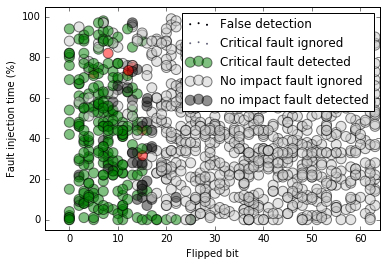
\includegraphics[width=1.1\linewidth]{figures/test_result_c05_0_full.png}
		\caption{$\varepsilon = 10^{-6}$}\label{fig:test_result_c05_0_full}	
	\end{subfigure}
    \quad
    \begin{subfigure}[t]{\linewidth}
		\centering
		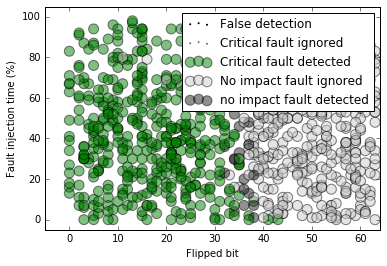
\includegraphics[width=1.1\linewidth]{figures/test_result_c05_1_full.png}
		\caption{$\varepsilon = 10^{-12}$}\label{fig:test_result_c05_1_full}	
	\end{subfigure}
    \end{minipage}
    \quad
    \begin{minipage}[b]{0.48\linewidth}
    	
	\begin{subfigure}[t]{\linewidth}
		\centering
		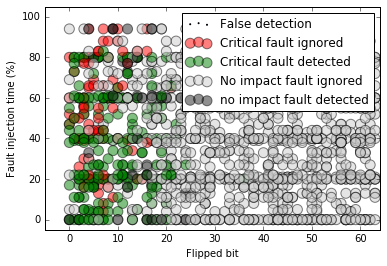
\includegraphics[width=1.1\linewidth]{figures/test_result_c05_0_precond.png}
		\caption{$\varepsilon = 10^{-6}$}\label{fig:test_result_c05_0_precond}	
	\end{subfigure}
    \quad
    \begin{subfigure}[t]{\linewidth}
		\centering
		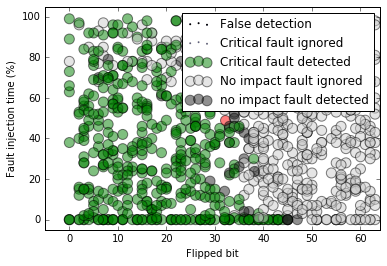
\includegraphics[width=1.1\linewidth]{figures/test_result_c05_1_precond.png}
		\caption{$\varepsilon = 10^{-12}$}\label{fig:test_result_c05_1_precond}	
	\end{subfigure}

	\end{minipage}
\caption{Diagram detailing the test results for $c = 0.5$ and several matrices. Each dot corresponds to a faulty execution, and its color represents the test outcome.}
\label{fig:test_result_c05_matrices}
\end{figure}





